\chapter{Lecture 11}
\chapterauthor{Kommireddy Bhargav Srinivas}

\section{Scope and Extent}
\subsection{Scope}
    Region of the code where the binding of the identifiers occur.
\subsection{Extent}
    During execution, the time duration in which the binding exists (not during the creation of closure but when the closure is called). Lexical scope can give you infinite extent.
\begin{verbatim}
> (define g
      (let ([x 2])
          (let ([f (lambda () x)])
             f))
\end{verbatim}
This returns a closure and the binding [x 2] is captured in the environment of the closure. So the extent of the binding will stay till g ends.

\section{DYNAMIC Language}
\subsection{Syntax}
Syntax is identical to LEXICAL
\subsection{Semantics}
Example:
\begin{verbatim}
> (define g
      (let ([x 5])
          (let ([f (lambda () x)])
             f))
> (g) ;; => 5
> (let ([x 2])
    (g)) ;; => 5 if LEXICAL, => 2 if DYNAMIC 
\end{verbatim}
The following are the evaluation semantics:

\begin{enumerate}
\item $\bigfrac{}{\Gamma \vdash \overline{n} \Rightarrow n}$ NUM
\item $\bigfrac{}{\Gamma \vdash \overline{b} \Rightarrow b}$ BOOL
\item $\bigfrac{\Gamma(x) = v}{\Gamma \vdash x \Rightarrow v}$ ID
\item $\bigfrac{}{\Gamma \vdash \lambda \overrightharpoonup{x} e \Rightarrow <\overrightharpoonup{x}, e>}$ ABS (Dynamic)
\item $\bigfrac{\Gamma \vdash e \Rightarrow <\overrightharpoonup{x}, e'>, \Gamma \vdash e_{i} \Rightarrow v_{i}, \{x_{i} \mapsto v_{i}\}\Gamma \vdash e' \Rightarrow v }{\Gamma \vdash @ e \overrightharpoonup{e_{i}} \Rightarrow v}$ APP CLOSURE (Dynamic)
\end{enumerate}

Shell Languages (eg: Sh, Bash, etc) have dynamic scope.

\section{RECURSION Language}
\subsection{Syntax}
$$
e ::= \overline{n} \quad | \quad \overline{b} \quad | \quad \textit{if e e e} \\
$$
$$
e ::= \textit{@ e e ...} \quad | \quad \lambda \textit{ } (x \dots) \textit{ } e \\
$$
$$
e ::= \textit{letrecfns } (fbind \dots) \textit{ } e 
$$
$$
fbind ::= [\textit{fid } (id \dots) \textit{ } e]
$$

Example:
\begin{verbatim}
(letrecfns ([f (x y) e_{1}]
              [g (a b) e_{2}])
            e)

;;; Factorial

(letrecfns ([f (n) 
                (if (= n 0)
                    1
                    (* n (f (- n 1))))])
            (f 2))
\end{verbatim}

\subsection{Semantics}

\begin{enumerate}
\item $\bigfrac{c = <\overrightharpoonup{x}, e, \Gamma>}{\Gamma \vdash \lambda \overrightharpoonup{x} e \Rightarrow c}$ ABS LEXICAL
\item $\bigfrac{\alpha = \{f_{i} \mapsto c_{i}\}, c_{i} = <\overrightharpoonup{x_{i}}, e_{i}, \Gamma>, \alpha\Gamma \vdash e \Rightarrow v}{(letrecfns \textit{ }(\overrightharpoonup{f_{i}, \overrightharpoonup{x_{i}}, e_{i}}) e \Rightarrow V)}$ LETRECFUNCS
\end{enumerate}

    \begin{figure}[htbp]
        \center
        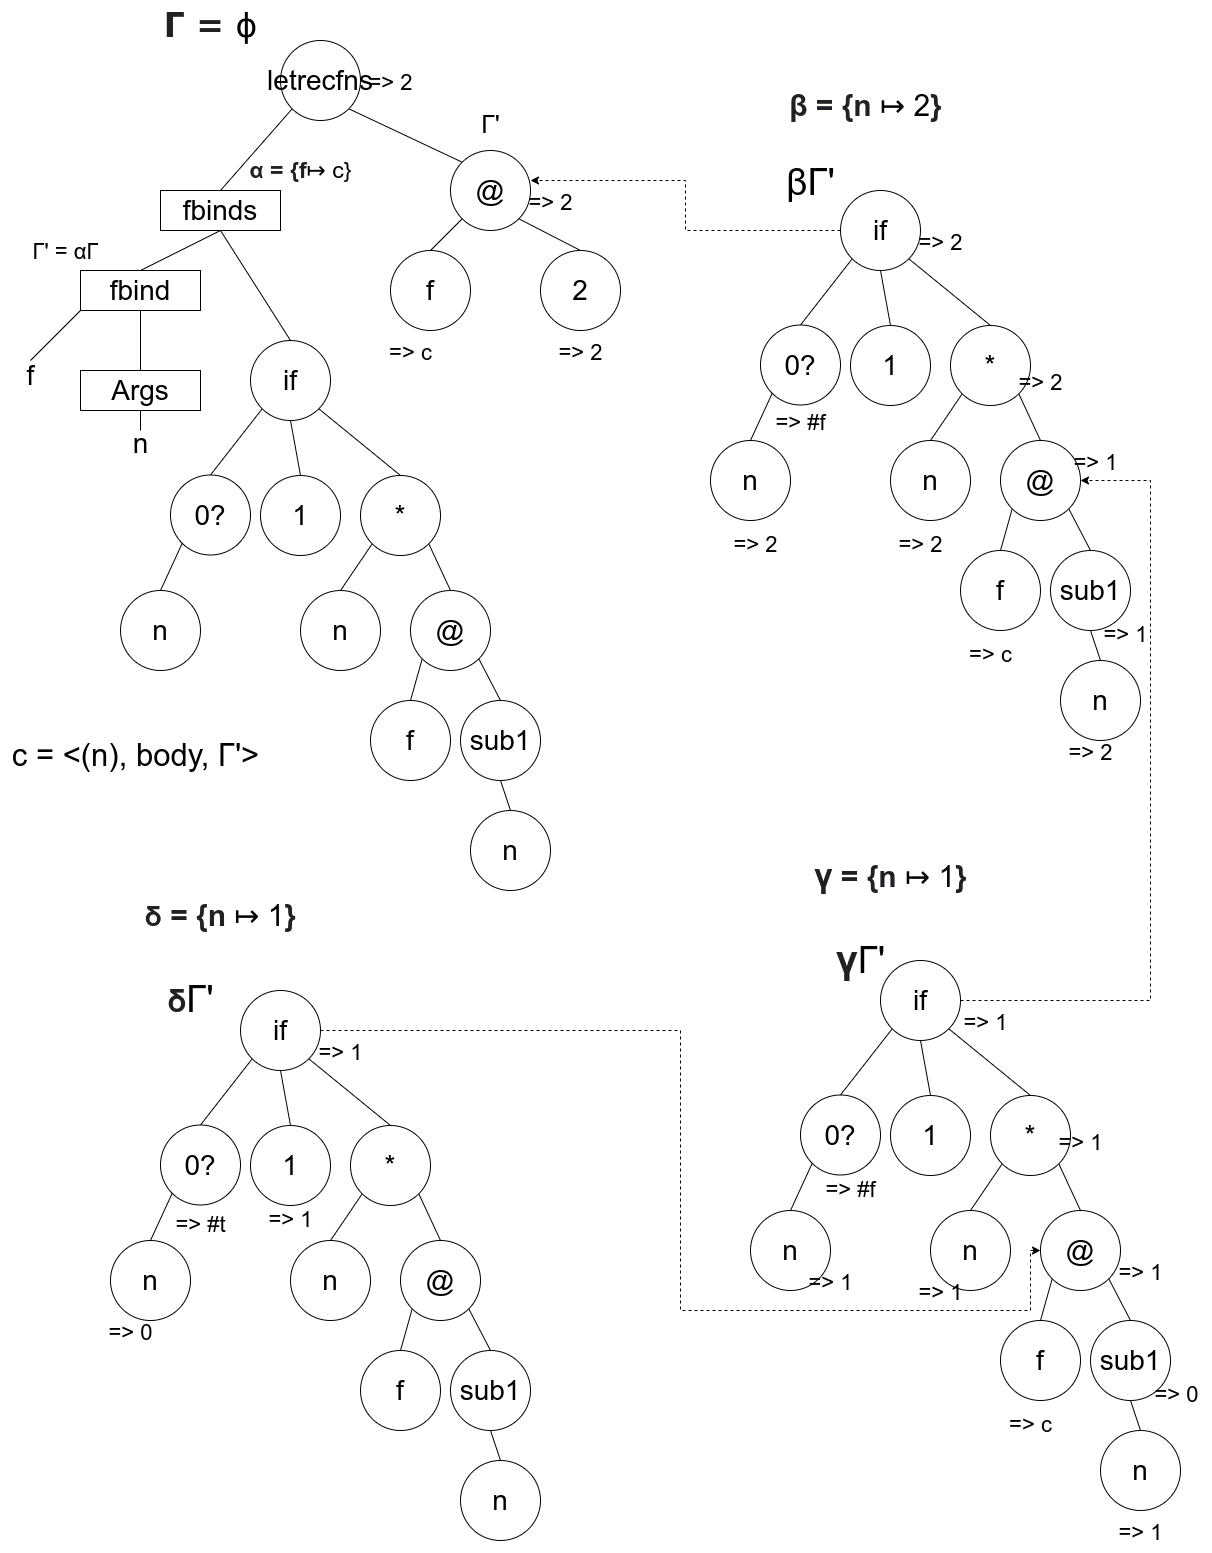
\includegraphics[scale=0.35]{images/lecture11/recursive_factorial.png}
        \caption{AST for Factorial using letrecfns}
    \end{figure}